\chapter{Mechatronic Design}

An ideal tensegrity system, either robotic or static, is a collection of rigid compressible elements suspended within a network of tensioned cables where non of the compressible elements are in direct contact with one another. 
For a robotic tensegrities without a payload, the actuation and supporting electronics would be logically designed into the compressible elements. 
For the inception of \SB{}, this compressible element was further dissected into three parts: two identical end caps (Modular Tensegrity Robots) and a section of tube stock.


%For \SB{}, the idea of making the compressible element  a self contained module that could be the coupled with another identical module  

%For SUPERball, each compressible element would be comprised of three parts: two identical end caps and a piece of tube stock. 
%Therefore, SUPERball can be thought of as a collection of identical robots (end caps) connected mechanically through rods and cables to enable entire system the ability to locomote.
%In this section, the main focus will be the mechatronic description of the end cap, with a focus on how each subsystem was designed to achieve an unteathered tensegrity for locomotion and system state research. 



\begin{figure}[thpb]
\begin{subfigure}{.5\textwidth}
      \centering
      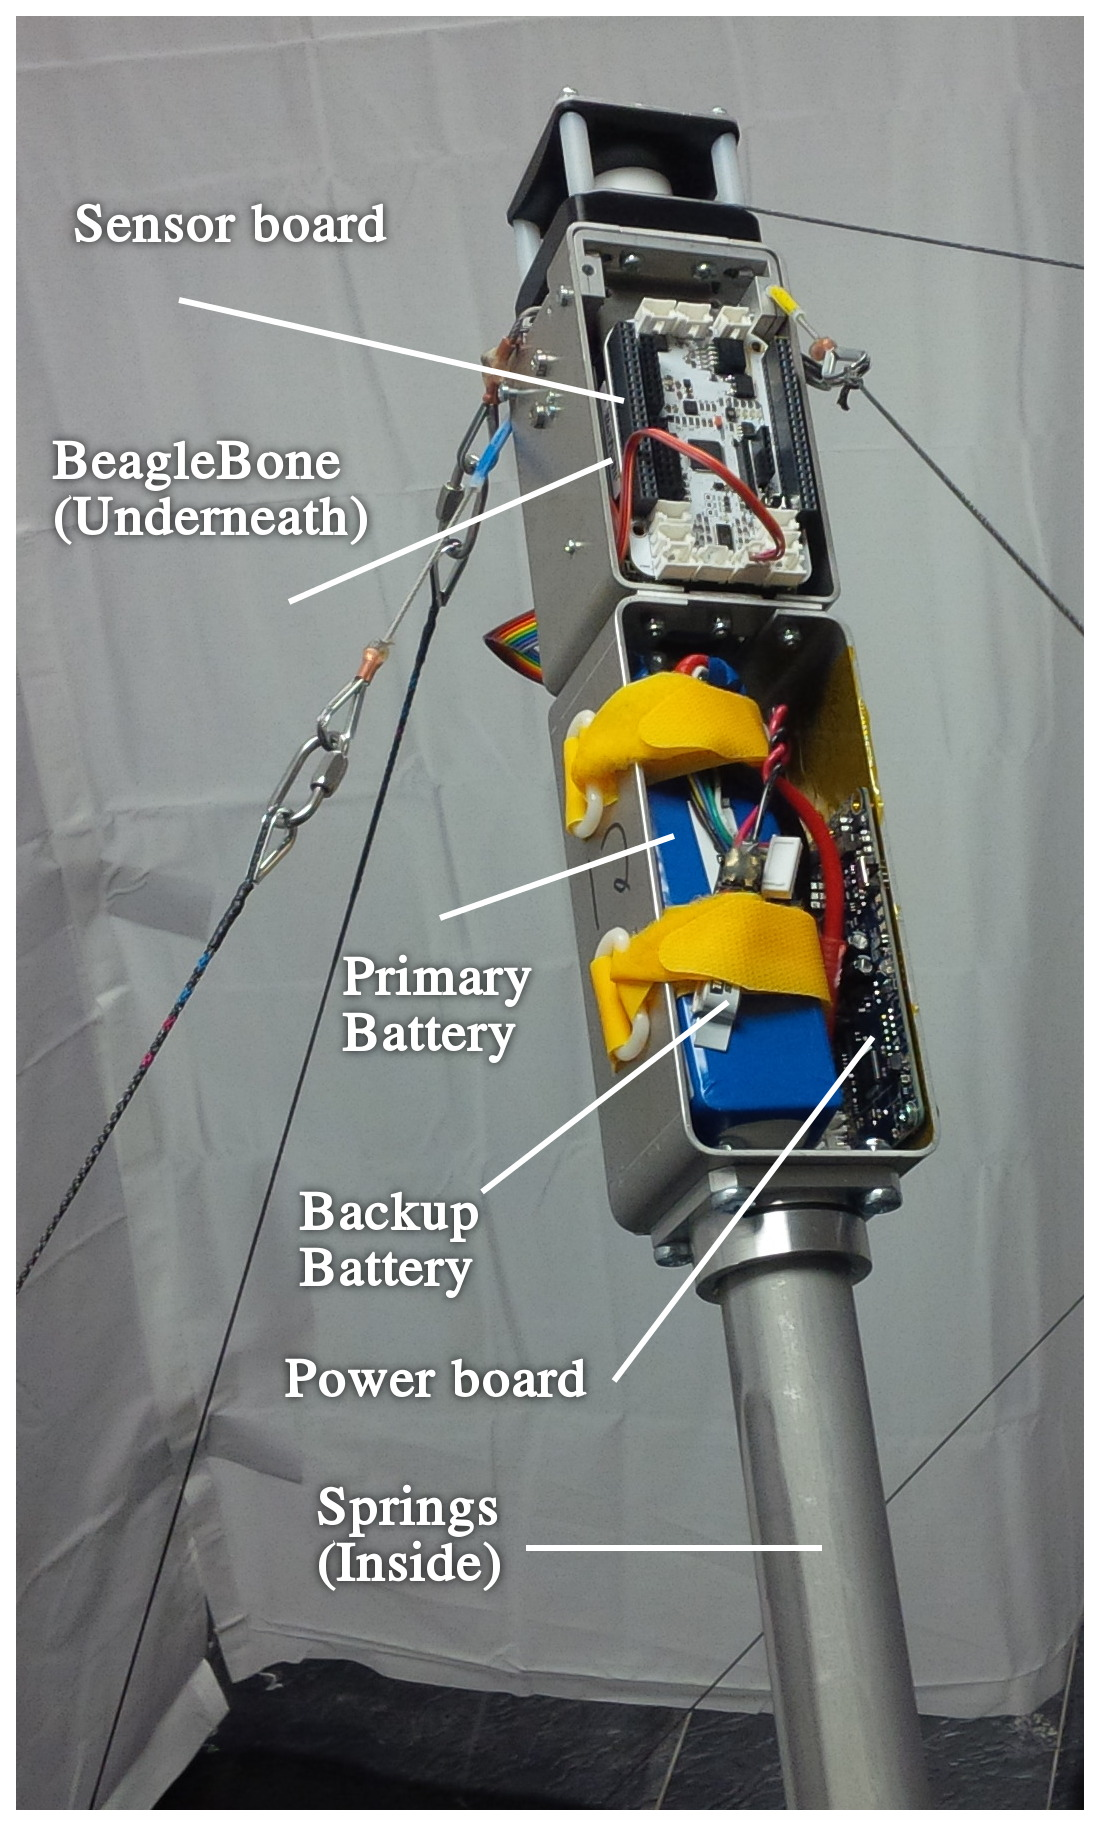
\includegraphics[width=0.5\columnwidth]{tex/img/endcap_upclose_sensorboard_labelled_fixedfonts}
      \caption{end cap front side.}
      \label{fig:endcap_upclose_front}
\end{subfigure}
\begin{subfigure}{.5\textwidth}
      \centering
      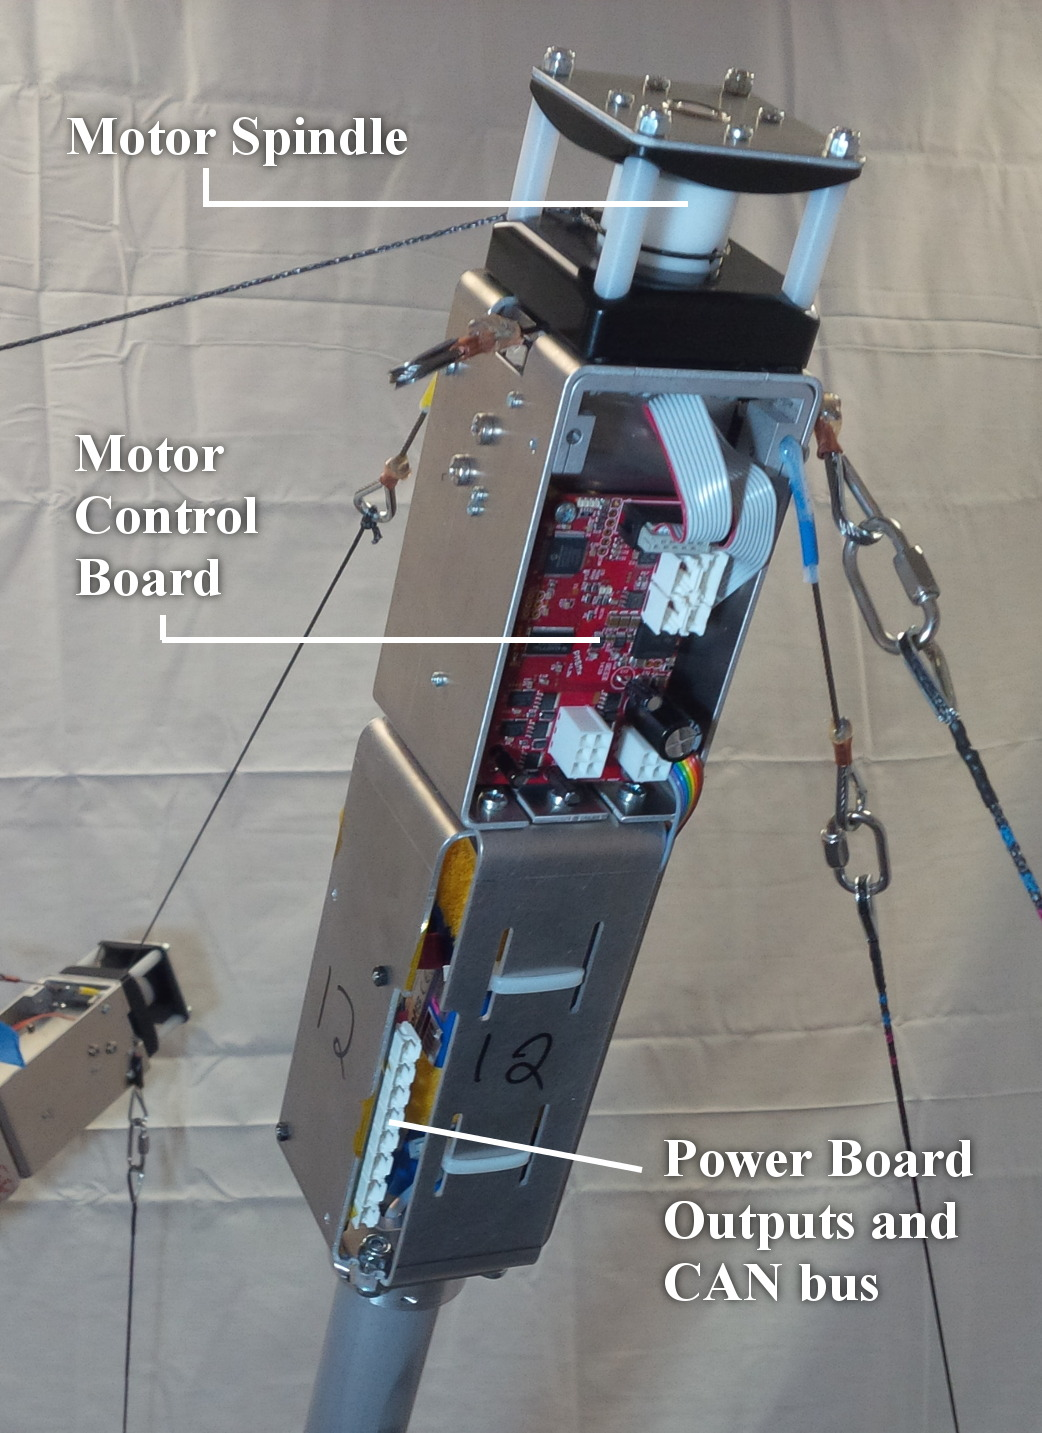
\includegraphics[width=0.5\columnwidth]{tex/img/endcap_upclose_motorboard_labelled_fixedfonts}
      \caption{end cap back side.}
      \label{fig:endcap_upclose_back}
\end{subfigure}
\caption{Fully assembled end cap images on SUPERball}
\label{fig:fully_assembled_endcap}
\end{figure}

\section{Mechanical}
Write about the mechanical design of SUPERball. Make sure to give credit where credit is due.

B.  Mechanical Design
The main structural elements of the end caps were
kept as  simple as possible and  in  sections  to  enable  each  end  cap  to  be self  contained  so  that  the  end  cap  may be removed from the connecting rod as one whole unit.
The end  caps  are  held  onto  the  connecting  rods  by  a  simple tube  collar  for  easy  removal. 
There  are  5  sections  to end cap: a spring holder, battery holder, motor and electronics, cable actuation and routing, and a ground contact. 
These sections as they are designed for SUPERball are shown in figure \ref{}. 
Design parameters, both ideal goals and built, are shown in table \ref{} **Table with design parameters!!**
For simplicity in manufacturing, the supporting structure is made from bent 6061-T6 aluminum sheet unless otherwise noted.

\subsection{Spring Holder}
A  lesson  learned  from other tensegrity robots and the designer of ReCTeR (reference) was  that  externally  exposed springs are not ideal for a robotic system that would be interacting with a dynamic and unknown enviroment. 
The exposed springs get caught on objects and the assumption of near mass-less cables  can  no  longer  be  applied.  
On  the  end  cap for SUPERball, an enclosed compression spring system was developed  to  alleviate  these  issues.  
Compression  springs were chosen so that during any unknown impact, the springs would not plastically deform without the need for any external hardware. 
For SUPERball, a spring with a spring constant of \(998 Nm\) is attached to a passive cable element  and  a \(2850 Nm\) spring  is  attached  to  an  actuated cable.  
A  passive  spring was chosen with a total throw of \(23 cm\) to allow for pretension to be instated into the passive springs as well as to allow a wide dynamic compliant range.  
Since the cables which are actuated will be able to dynamically control the pretension, a smaller throw spring was chosen to conserve space.

\subsection{Battery Holder}
\label{battery_holder}
From the inception of SUPERball, enabling a self-contained power source which was easily accessible per end cap was a driving design parameter.
During the initial design and build of SUPERball, It was known that the batteries where to be 24 volt lithium polymer but optimal size and shape of the battery was unknown due to a changing power profile.
Therefore, a battery holder with a simple securing mechanism which can handle a wide range of battery sizes was utilized.
Two hook and loop straps where used with simple slot cutouts to enable cinching around a generic lithium polymer battery.
The holder was also made large enough to hold the Power Board PCB board opposite of the battery.
As shown in section \ref{power_board}, the Power Board was designed to be an low profile to allow for a large battery within the holder.
Figure \ref{}**reference a picture of just the battery holder** shows a the battery holder as designed on SUPERball.

\subsection{Motor and Electronics}
\label{mechanical:motor}
This section of SUPERball was mechanically designed around the Maxon EC-22 100 watt BLDC motor used for actuation. 
Each Maxon motor is \(22 mm\) in diameter and \(108 mm\) long with gearbox and encoder.
The output shaft is a \(6 mm\) in diameter D shaft of length \(10.2 mm\).
A size requirement for how large the cross sectional diameter of the end cap could be was quite a limiting factor in designing the motor and electronic section.
The maximum diameter for any section used in the end cap was maximally limited to double the diameter of the connecting rod.
The idea for such a limitation was to keep the effective moment arm out from the center axis of any rod to a minimum.  
Due to the spring size and the need for a spring holder tube, the minimum diameter for the connecting rod was \(~35mm\) giving a maximum end cap diameter of \(70mm\).

The main component in the motor and electronic section of the end cap, is the cable routing support bracket. 
This bracket plays three roles in the mechanical design: static support for the motor, support for the supporting material, and main exit support for the internal cable routing.
Figure \ref{} **figure of the cable routing supporting bracket** shows the cable routing support bracket.
The actual motor mount was designed to be mechanically floating to enable torque sensing directly on the motor mount.
Thus, the cable routing support bracket sinks the reaction torque induced by the motor.
The motor mount bracket with torque sensor can be seen in figure \ref{}.
There are two electronic boards, the Sensor and Motor boards, which are mounted to brackets that straddle the motor.
Due to space limitations, these brackets are also load bearing components for the torsional forces induced by the motor.
Figure \ref{} **reference the main figure for the end cap** shows one of the brackets with the corresponding electronic board mounted.

\subsection{Cable Actuation and Routing}
A simple spool design was implemented to directly actuate the cable. 
The spool directly couples to the motor shaft by press fitting onto the D shaft.
The force vector applied to the spool by the actuated cable will never be perpendicular to the spool, therefore a thrust bearing was embedded into the spool and a radial bearing supports the top of the spool.
For completeness, spool has the ability to slide along the the shaft's main axis and the thrust bearing sinks the trust force into the motor mount.
Since this thrust force is perpendicular to the torque of the motor, this force is not induced into the torque sensor built into the motor mount.
Figure \ref{} shows the spool with thrust bearing cutout and radial bearing.

There are three other cables that connect to an end cap.
Two are routed through the end cap to the spring housing section and the other is terminated on the end cap.
The cables used externally from the end cap is composed of Vectran braided cable and the cables used within the end cap are braided steel cabling. 
Both routed cables enter the end cap through the cable routing support bracket mentioned in \ref{mechanical:motor}.
The cables are immediately routed around a rolling guide bearing to induce an approximate 90 degree bend to guide the cables towards the spring tube holder section.
After the rolling guide bearing, the cables enter a PTFE tube to create a type of bowden cable to help route the cables around components within the end cap.
Once the cables reach their respective spring within the spring tube holder, the PTFE tube is terminated and the cable is routed through the spring and terminated using a copper compression sleeve.

\subsection{Ground Contact} 
This final section of the end cap is the simplest. 
To protect the end cap during locomotion, a 3D printed cap was manufactured to cover the end.
This part is designed so that it is the only part of the end cap that contacts the ground during normal locomotion.
To decrease the impact shocks as the rod contacts a surface, compliant foam sheets are place between the 3D printed cap and the end cap.
Figure \ref{} shows the 3D printed cap and the foam sheets.

\section{Electrical}
\SB{}'s electronics where developed with a focus on reliability, safety, and enabling distributed controls.
Another parameter was the ability to drive the 100W BLDC Maxon motors (see section \ref{mechanical:motor} for detailed information on this motor).
These main design criteria gave way to implement separate electronic boards per end cap based on their main function.
Each end cap has three custom Microchip dspic33e enabled PCB boards and only one end cap per rod has an ARM based computer called a Beagle Bone Black.
Each custom PCB is designed for very different purposes: A board to condition sensor data and run real-time control loops, a board to condition and distribute a 5.5V electronic power rail and a 24V motor power rail, and a board to control the 100W BLDC motor. 
The only requirements for each custom board is full CAN bus communication and power conditioning required for the 5.5V power rail.
The boards are simply named by their main purpose, thus Sensor, Power, and Motor respectively.

\subsection{Motor Board}
An initial driving parameter used during the design of SUPERball was the BLDC motor. 
During the design review for \SB{}, a lightweight motor with high power and efficiency was wanted.
Thus, a Maxon brushless motor was a logical choice (see section \ref{mechanical:motor} for detailed information on this motor).
In order to effectively drive this motor, a dedicated motor board was used on each end cap.
The main development of this board was engineered by Pavlo Manovi, and certain aspects of the board where tailored for our needs \ref{}.
The main components on the Motor board are the Microchip's 16-bit dsPIC33ep256mu506 micro-controller and the Texas Instruments DRV8303 three phase pre-driver.
Figure \ref{} shows the current version of the motor board.

\subsection{Sensor Board and Beagle Bone Black}
\label{sensor_bbb}
The sensor board was originally designed as the main processing unit on an end cap for \SB{}. 
However, the design and building process has lead to the coupling of the sensor board with a Beagle Bone Black.
For a detailed explanation of why the Beagle Bone Black was integrated into the system, please refer to \ref{communication}.

The current version of the sensor board was developed as a daughter board for Beagle Bone Black \ref{}.
The board mates to the Beagle Bone Black through two double row 46 pin headers and provides power and CAN communication to the ARM board.
The main processing unit on the sensor board is Microchip's 16-bit dsPIC33ep128gp506 micro-controller.
Environmental sensing is enabled through a 9DOF inertial measurement unit (IMU) and a 24-bit analog to digital converter (ADC) configured in a half wheat-stone bridge configuration.
The IMU is comprised of Invensense's MPU6000 mastered to Freescale's MAG3110 magnetometer, and the ADC is Analog Device's AD7193.

The Beagle Bone Black is a open-source hardware single-board computer inspired by the BealgBoard, the larger predecessor developed by Texas Instruments as an educational tool.
The main processor on the board is a Sitara ARM Cortex-A8 processor running at 1Ghz and capable of running a full ARM based operating system.
The processor is also able to interface directly with low level communication protocols such as CAN, UART, SPI, and I2C.
To meet our memory and speed requirements, a custom kernel was built with only the main modules needed by our system.
On top of this kernel, the Beagle Bone Black is running a ROS (Robot Operating System, see section \ref{communication} for more detials) enabled Ubuntu ARM 14.04.1 LTS operating system.

A new feature still being developed is the integration of DecaWave's DWM1000 module for relative distance measurements.
Legacy components no longer utilized on the sensor board are mounting pins for an XBee device.
A small breakout was designed to integrate the DWM1000 module into where the XBee device was originally mounted.
Figure \ref{} shows the sensor board mounted to a Beagle Bone Black and the DWM1000 module.

\subsection{Power Board}
\label{power_board}
The power board was design to enable safety, both for a person working near \SB{} and for the electronics, as well as conditioning input power to both a 5.5V and a 24V rail.
The board was also designed with a minimal height profile allowing for larger batteries to be placed near the board.
See section \ref{battery_holder}, to view the section which houses the power board.
The main idea of safety is focused around operating the 100W BLDC motors, thus a two battery system was implemented.
A small battery used for starting the micro-controller boards but not capable of producing 24V needed by the motor, and a large battery used during main operation of the end cap.
The two batteries used are a 160 milli-amp-hour 1-cell and a 3 amp-hour 6-cell lithium polymer batteries, named the back-up and the main receptively.
To enable the 24V power, multiple input conditions should be met fed into an analog and-gate.
The input conditions are: a physical switch located on the end cap, a digital logic pin from the power board's micro-controller, power being applied by the back-up battery, and a signal coming from a dedicated 8-bit micro-controller monitoring a pulsed wireless 2.4Ghz signal.
If any one of these conditions go false, then the full 24V rail is disabled.
There are also fuses on both the 24V and 5.5V line to protect all the micro-controller circuits from shorts.
Figure \ref{fig:connection_diagram} shows a basic connection diagram for the power lines.

The main processing unit on the power board is Microchip's 16-bit dspicPIC33ep128mc506 mirco-controller.
The wireless "kill switch" monitoring mirco-controller is Mircochip's 8-bit PIC12(L)F1571/2 mirco-controller.
This chip monitors a known pulse width being communicated by a Nordic Semiconductor nRF24L01 breakout board with antenna.
The pulsed signal is sent by a hand held unit off the robot.
When a shut off command is sent or the PIC12's watchdog timer is triggered from a delay in wireless signal, the logic signal sent from the PIC12 is turned to false disabling the 24V power rail. 
5.5V power is either supplied by the back-up battery or the main battery using a custom boost or buck switching circuit, receptively.
The 24V rail is supplied directly from the main battery when all input logic is enabled.
Figure \ref{} shows the power board with nRF24l01 chip mounted. 

\section{Communication and Power}
\label{communication}

Communication on \SB{} was designed around a desire to have each rod of the tensegrity system unteathered from any other part of the system.
Two wireless protocols as well as a wired Controller Area Network, or CAN, bus were implemented.
The two main wireless protocols are WiFi for main data communication and a 2.4GHz channel for wireless switching power for safety.
Figure \ref{fig:connection_diagram} shows how power and communication are connected for a single end cap and figure \ref{fig:ros_diagram} shows the connections for \SB{}'s wireless communications.

\begin{figure}[thpb]%{.5\textwidth}
      \centering
      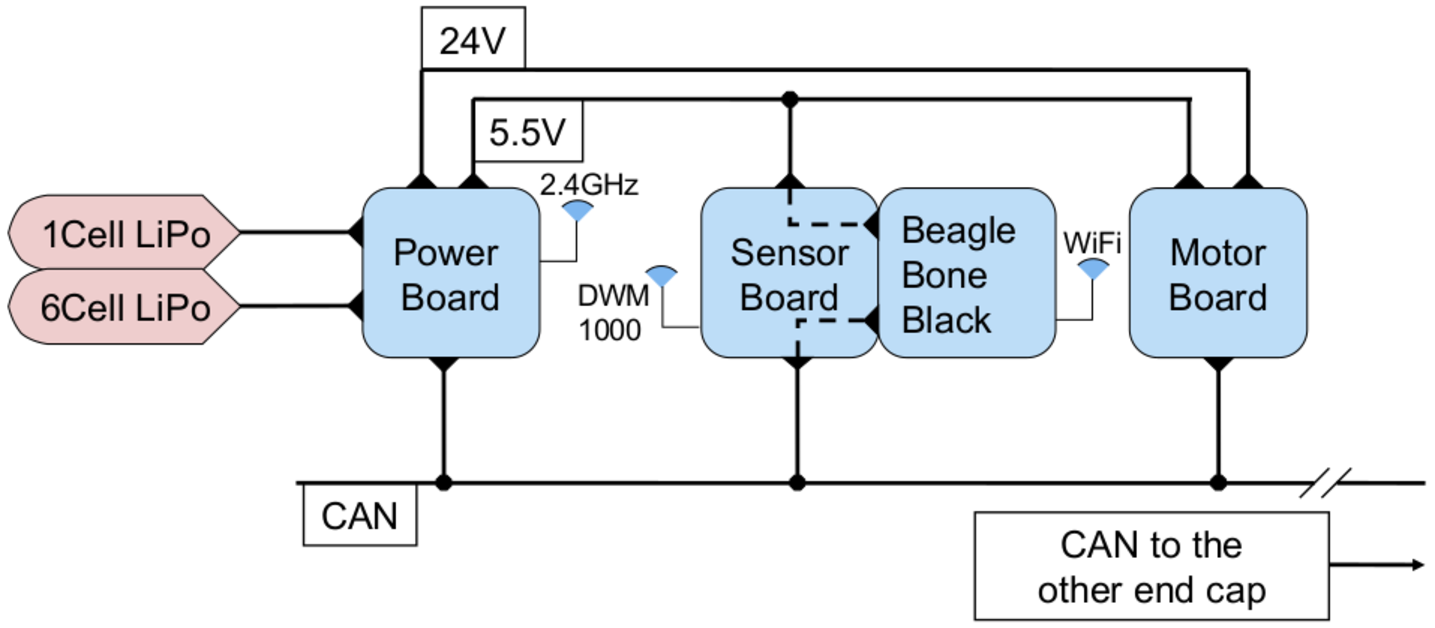
\includegraphics[width=0.8\columnwidth]{tex/img/hard_wire_connection}
      \caption{This is a connection diagram for power and communication for an end cap on \SB{}.}
      %\vspace{-0.5cm}
      \label{fig:connection_diagram}
\end{figure}

\subsection{CAN Bus}
A communication design was desired that would be robust, extensible, and work over long distances.
A CAN bus fits these main requirements and was implemented to be the main communication between all controllers on a single rod.
Since the CAN bus is a physical layer standard, a communication protocol is usually required to get a robust and extensible network.
A widely accepted protocol that has been well tested and understood, is the CANOpen protocol \ref{}.
CANOpen defines the addressing scheme, several small communication protocols and an application layer defined by a device profile.
Some of the smaller communication protocols supported by CANOpen are device monitoring and communication between nodes, network management, and a simple transport layer for message processing.
This open source protocol is freely distributed and has many open and closed source implementations.
The CANOpen implementation used for \SB{} is the CANFestival project which focuses on implementing the basic protocol while maintaining a small code base and low computational load for embedded systems \ref{}.
Each mirco-controller and Bealge Bone Black are able to run the entire CANFestival project code in less than \(150 \mu s\) under worst case scenarios.
The physical layer CAN bus is running at \(1 Mbit/s\) 

\subsection{WiFi and the Robot Operating System}
The Robot Operating System, or ROS, is a collection of software to provide operating system functionality on a network linked computer cluster. 
Message-passing and packet management works agnostic to the network layer, allowing information to be passed from one ROS enabled node to any other ROS enabled node on a network.
Figure \ref{fig:ros_diagram} shows a basic representation of how this message-passing works on the \SB{} ROS network.

As explained in section \ref{sensor_bbb}, enabling each rod is a ROS node was the driving reason to have at least one ARM based chip on every rod.
Since the Beagle Bone Black is also on the CAN bus, it's main function is to sniff the CAN network and send new information out to the ROS network.
This enables for near real time data analysis and for time stamped data logging on \SB{}.

\begin{figure}[thpb]%{.5\textwidth}
      \centering
      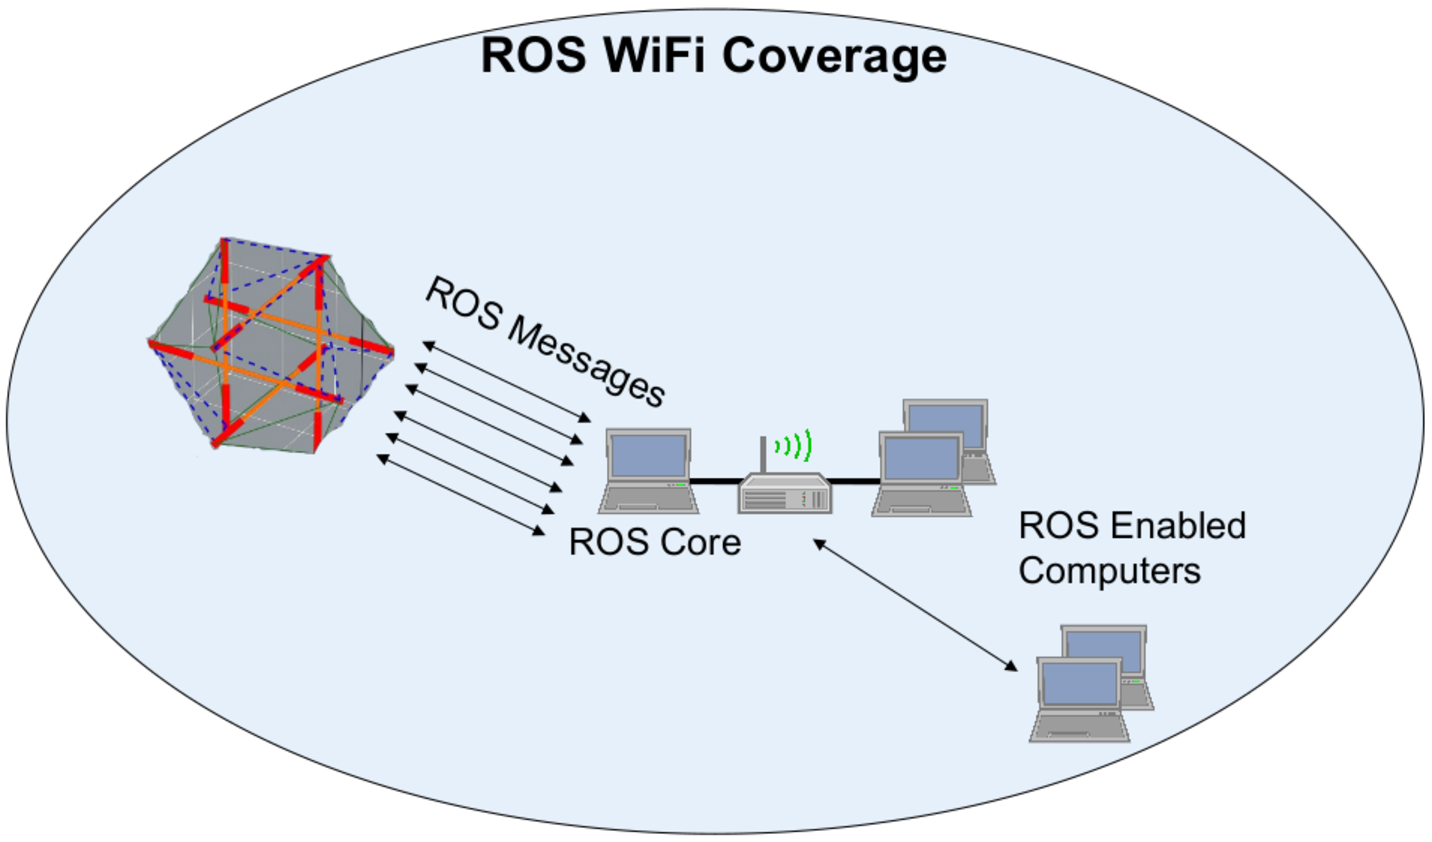
\includegraphics[width=0.8\columnwidth]{tex/img/ROS_Wireless}
      \caption{A simplified representation of how messages are passed within the \SB{} ROS network.}
      %\vspace{-0.5cm}
      \label{fig:ros_diagram}
\end{figure}
